% !TeX encoding=utf8
% !TeX spellcheck = de_CH_frami

\section*{Abstract}

%\todo{Abstract, Abstract Template: ZHAW\_FUP\_SEM\_IOT\_Abstract.tex}
\subsection*{Ausgangslage und Ziel}
Einer immer grösseren Beliebtheit erfreuen sich kleine Alltagsgegenstände welche mit dem Internet verbunden sind, genannt \gls{acr:IOT}. Diese Geräte sind in der Lage Daten zu sammeln und weiterzuleiten. Da es zukünftig immer mehr solcher Geräte geben wird fallen immer mehr Daten an. Der Themenbereich des Aufbereiten, Aggregieren, Analysieren und Visualisierens dieser Daten wird auch als "`BigData"' bezeichnet.

Das Hauptziel dieser Arbeit ist die Überprüfung, ob sich funktionale Programmiersprachen eigenen um Sensor-Daten auf einem \gls{acr:IOT} Gerät zu sammeln und anschliessend auszuwerten. Um diesen Sachverhalt zu prüfen, sollen mit einem \gls{acr:IOT} Gerät (Raspberry Pi) Sensor-Daten ermittelt und anschliessend aufbereitet und visualisiert werden.

\subsection*{Sensordaten sammeln}
Als erstes mussten Daten mit einer Raspberry Pi gesammelt werden. Um dies zu bewerkstelligen wurde parallel zwei Betriebsysteme für dieses \gls{acr:IOT} Gerät getestet. Dies wären Raspbian und Windows 10 IoT. In diesem Kapitel werden die Probleme bei der Inbetriebnahme des Raspberry Pi erläutert und tiefe Einblicke in dessen Programmierung gegeben.

\subsection*{Sensordaten aufbereiten und auswerten}
Der zweite Schritt der Arbeit ist es, die Daten darzustellen und die Eignung von F\# in Bezug auf BigData zu prüfen. Zum auslesen der Daten wurde F\# Data verwendet und zur Darstellung FSharp.Charting. Um die Daten zu abstrahieren und in die richtige Form zu kriegen wurde herkömmlicher F\# Code verwendet.

\subsection*{Resultat}
Das Endresultat besteht aus einem lauffähigen Raspberry Pi und einem Programm für die Darstellung der Daten.
\begin{figure}[htb]
	\begin{subfigure}[b]{0.45\linewidth}
		\centering
		\includegraphics[width=6.5cm]{images/_DSC2012}
		\caption{Raspberry Pi mit GrovePi Board und Sensoren}
	\end{subfigure}
	\begin{subfigure}[b]{.45\linewidth}
		\centering
		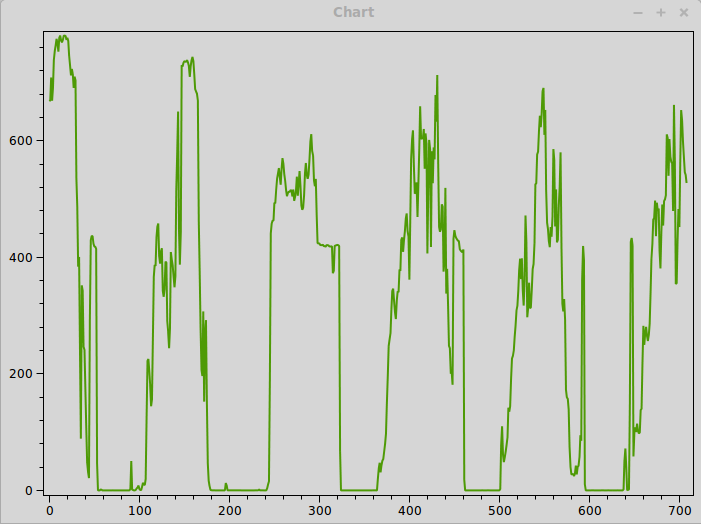
\includegraphics[width=6.5cm]{images/resultat}
		\caption{Visualisierung der Daten}
	\end{subfigure}
\end{figure}
